\section{Results}
\label{sec:results}

\subsection{Certified coverage}
\label{sec:main}

Table~\ref{tab:main} compares CCRC with filtering on identical folds at $\alpha\in\{0.10,0.15\}$,
$\delta=0.10$, all items, and Figure~\ref{fig:forest} plots the gains with their bootstrap intervals. Three
certified gate variants appear. In the \emph{external} variant the gate fraction $q$ is a constant chosen once on a
different benchmark (AMBER for the POPE cells, POPE-3000 for AMBER), by running the same protocol there on random
subsamples whose calibration fold has the \emph{target's} size and keeping the candidate (filtering, or
$q\in\{0.05,0.10,0.25,0.50\}$) with the highest mean certified coverage. The choice is $q=0.05$ for
the small cells at $\alpha=0.10$, the small LLaVA cell at $0.15$ and POPE-1500 at $0.10$ ($q=0.05$ in five of the twelve combinations) and $q=0.5$ in the other seven. In the \emph{fit-fold}
variant $q$ is chosen inside each split on the fit fold, with filtering as one candidate. A third variant
(\emph{external, full-size}) treats the whole development benchmark as a single calibration sample; it is
reported in the last column of Table~\ref{tab:main} because it shows what picking the gate at the wrong
sample size costs. The size-matched variant was defined after we saw that the full-size variant loses on the small cells, so
the comparison between them is exploratory and the size-matched rule should be read as a recommendation.

\begin{table}[t]
\centering
\caption{Certified coverage (\%), with the abort rate (\%) in parentheses, $\delta=0.10$, $400$ paired
splits, all-item cohort. Gain is the mean paired difference over splits against filtering; the interval is the
$95\%$ percentile interval from the outer image-level bootstrap (\S\ref{sec:protocol}), and
$P(\text{gain}>0)$ is the fraction of bootstrap datasets with a positive gain. The last column is the gain with the
gate chosen on the development benchmark at its full size.}
\label{tab:main}
\scriptsize
\resizebox{\textwidth}{!}{\begin{tabular}{lcccccccc}
\toprule
 & & Filter & \multicolumn{3}{c}{CCRC, external gate} & & \multicolumn{2}{c}{CCRC, fit-fold gate}\\
\cmidrule(lr){4-6}\cmidrule(lr){8-9}
Setting & $\alpha$ & cov.\ (abort) & cov.\ (abort) & gain [95\% CI] & $P(\text{gain}>0)$ & & cov.\ (abort) & gain [95\% CI]\\
\midrule
POPE-1500, LLaVA & 0.10 & 68.2 (0) & 71.1 (0) & +2.9 [+1.4, +11.8] & 0.99 & 77.0 (1) & +8.8 [$-$8.0, +18.8]\\
 & 0.15 & 85.5 (0) & 91.3 (0) & +5.8 [+1.3, +9.3] & 0.98 & 92.6 (0) & +7.1 [+3.6, +10.7]\\
\addlinespace
POPE-adv, LLaVA & 0.10 & 44.5 (25) & 48.2 (22) & +3.7 [$-$2.3, +10.3] & 0.91 & 41.4 (34) & $-$3.1 [$-$13.8, +9.3]\\
 & 0.15 & 72.5 (2) & 80.5 (2) & +7.9 [$-$5.9, +29.0] & 0.92 & 82.0 (2) & +9.4 [$-$3.3, +28.8]\\
\addlinespace
POPE-adv, Qwen2-VL & 0.10 & 76.9 (1) & 79.4 (0) & +2.6 [$-$1.5, +9.5] & 0.95 & 71.2 (10) & $-$5.7 [$-$25.1, +10.5]\\
 & 0.15 & 94.6 (0) & 95.4 (0) & +0.8 [$-$13.1, +10.7] & 0.70 & 95.0 (0) & +0.4 [$-$7.5, +8.9]\\
\addlinespace
POPE-adv, LLaVA+VCD & 0.10 & 45.8 (14) & 47.8 (11) & +2.0 [$-$1.9, +7.2] & 0.91 & 39.6 (30) & $-$6.2 [$-$13.4, +8.9]\\
 & 0.15 & 74.4 (0) & 76.0 (1) & +1.6 [$-$10.4, +20.5] & 0.76 & 76.1 (0) & +1.7 [$-$10.3, +17.6]\\
\addlinespace
AMBER(d), LLaVA & 0.10 & 55.2 (3) & 56.3 (6) & +1.1 [$-$15.1, +11.5] & 0.65 & 55.8 (6) & +0.6 [$-$8.5, +9.1]\\
 & 0.15 & 74.1 (0) & 76.1 (0) & +1.9 [$-$10.6, +7.9] & 0.73 & 75.3 (0) & +1.2 [$-$8.0, +5.9]\\
\bottomrule
\end{tabular}
}
\end{table}

\begin{figure}[t]
\centering
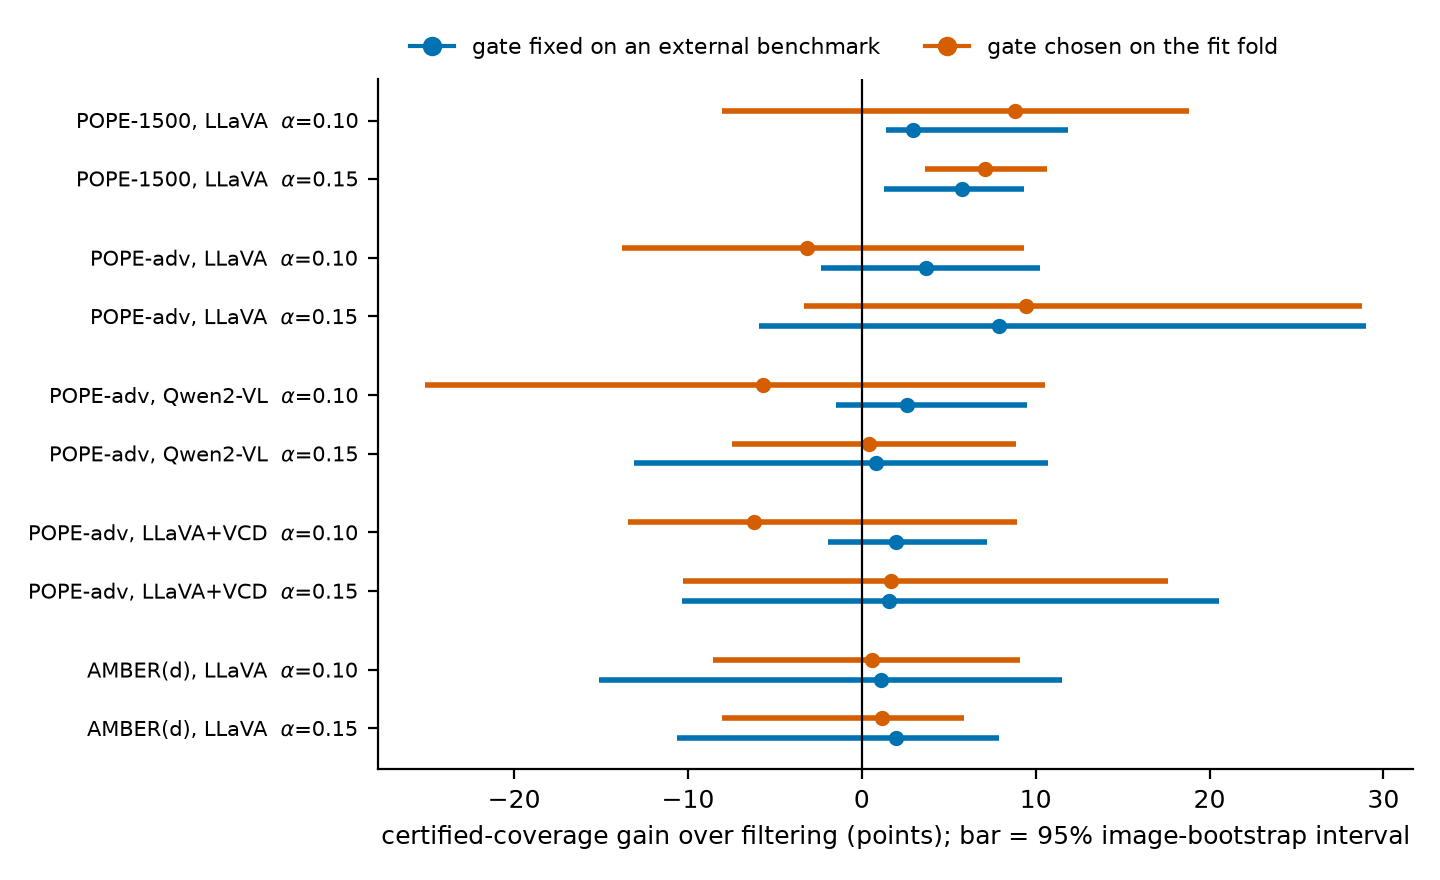
\includegraphics[width=0.9\textwidth]{fig_forest.png}
\caption{Gain in certified coverage over filtering. Points are means over $400$ splits of the original
benchmark; bars are $95\%$ image-bootstrap intervals.}
\label{fig:forest}
\end{figure}

With the size-matched external gate the gain is positive in all twelve (cell, $\alpha$) combinations, from $+0.8$ to
$+7.3$ points, and the share of bootstrap datasets with a positive gain is $0.60$--$1.00$. The $95\%$
interval excludes zero in seven of the twelve: POPE-1500 and POPE-3000 at $\alpha=0.15$, POPE-1500 at $0.10$, AMBER at $0.15$, and
three of the small cells, where the gain is $+1.2$ to $+1.8$ points with intervals whose lower end is within $0.15$ points of zero. The larger
gains occur where the calibration folds are large and the gate is $q=0.5$: $+6.6$ and $+5.1$ points on
POPE-3000 (folds of about $1000$ items, $166$ images), $+7.3$ on POPE-1500 at $\alpha=0.15$ and $+3.9$ on AMBER
at $\alpha=0.15$. On the small cells the selected gate is $q=0.05$, which repairs $0.2$--$0.7\%$ of test items and
gains about one point; the per-split standard deviations of the gain are $1.3$--$11$ points.

The fit-fold gate is more flexible and more variable: $+8.8$ and $+7.1$ points on POPE-1500 and $+6.3$, $+5.0$ on POPE-3000,
but between $-6.2$ and $+9.4$ on the small cells, negative in all three at $\alpha=0.10$, because a gate chosen
on a fit fold of $150$ items is itself noisy and a wrong choice costs more than the right one returns. The union over
three gates avoids selection noise and pays $\delta/3$ per gate: it gains $+2.0$ to $+4.4$ points on the
cells with $500$ or more calibration items and loses up to $16.5$ points on those with $150$--$200$
(Appendix~\ref{app:audit}). The full-size external gate ($q=0.5$ for every POPE cell) loses $7.2$, $7.7$ and
$12.3$ points on the three small cells at $\alpha=0.10$ and $5.5$ on AMBER at $0.10$, and gains up to $+10.1$ elsewhere. The continuity gate $q=0.10$,
selected in exploratory runs on these benchmarks, gains $0.0$ to $+3.9$ points; we report it as an uncertified reference arm
and do not use it for any claim, since a gate chosen with knowledge of the benchmarks is what
Theorem~\ref{thm:validity} does not cover.

\begin{figure}[t]
\centering
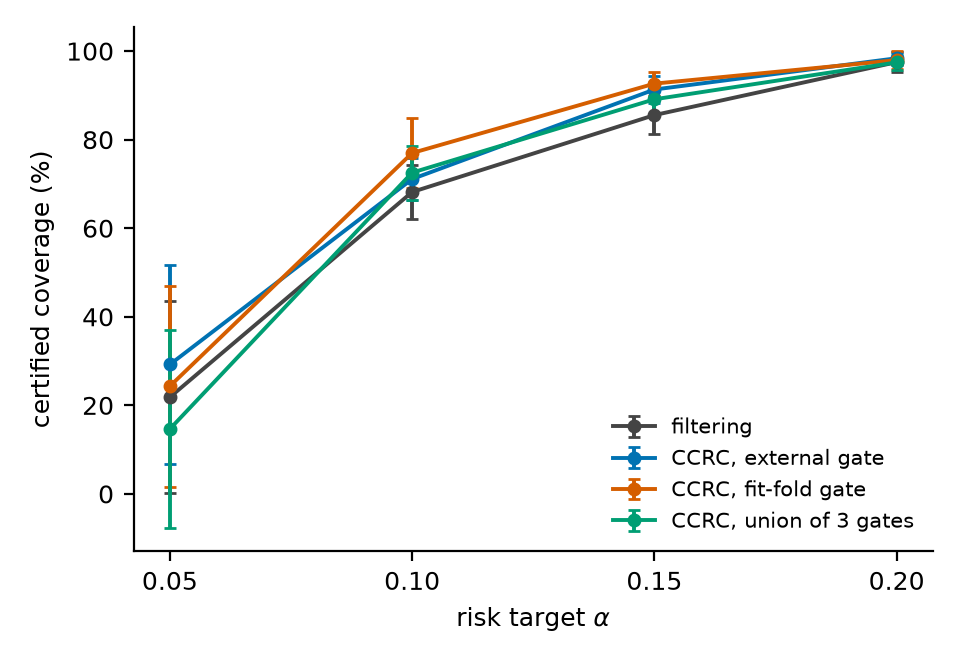
\includegraphics[width=0.55\textwidth]{fig_alpha.png}
\caption{Certified coverage against the risk target on POPE-3000. Bars are one standard deviation over
splits.}
\label{fig:alpha}
\end{figure}

Coverage rises with $\alpha$ for every arm (Figure~\ref{fig:alpha}), and the gap between CCRC and filtering is
largest at moderate targets. The audit columns of Appendix Table~\ref{tab:audit} are discussed in
\S\ref{sec:validity-audit}.

\subsection{What each protocol change does}
\label{sec:ladder}

Table~\ref{tab:ladder} introduces the changes one at a time, from a conventional implementation (item-level folds,
thresholds and gate as quantiles of the calibration fold, a start at $k_{\mathrm{start}}(0)$ and a fixed $q=0.10$) to the
protocol of this paper; the $\alpha=0.15$ version is in Appendix~\ref{app:ladder}.

\begin{table}[t]
\centering
\caption{Filtering / CCRC certified coverage (\%) at $\alpha=0.10$ as the protocol changes. Rungs L0--L3 use the
fixed gate $q=0.10$, rung L4 chooses the gate on the fit fold, and rung L5 keeps items with no detector
value. L0--L4 use the grounded cohort of each cell; L5 uses all items, so
its absolute level for AMBER is lower: the attribute and relation queries are harder and cannot be repaired.}
\label{tab:ladder}
\small
\resizebox{\textwidth}{!}{\begin{tabular}{lccccc}
\toprule
 & POPE-1500,\ LLaVA & POPE-adv,\ LLaVA & POPE-adv,\ Qwen2-VL & POPE-adv,\ LLaVA+VCD & AMBER(d),\ LLaVA\\
\midrule
conventional protocol (item folds, calibration quantiles, $e_0{=}0$, fixed $q{=}0.10$) & 68.6/71.8 & 44.0/47.1 & 77.9/79.7 & 48.8/51.0 & 91.8/81.6\\
+ image-grouped folds & 68.2/71.3 & 43.1/48.3 & 77.6/79.5 & 47.9/50.8 & 92.0/81.9\\
+ fixed value grid and gate (fit fold) & 67.5/70.9 & 35.0/42.3 & 75.5/77.7 & 39.9/45.3 & 90.9/85.1\\
+ analytic start $e_0{=}1$ & 68.2/71.1 & 43.6/47.4 & 75.6/78.0 & 45.5/47.6 & 90.2/90.0\\
+ gate chosen on the fit fold & 68.2/77.0 & 43.6/39.4 & 75.6/68.3 & 45.5/39.7 & 90.2/89.8\\
+ all-item cohort & 68.2/77.0 & 44.5/41.4 & 76.9/71.2 & 45.8/39.6 & 55.2/55.8\\
\bottomrule
\end{tabular}
}
\end{table}

Image-grouped folds change coverage by at most $1.2$ points on the POPE cells and lower the test-fold exceedance on the five
POPE cells from $0.14, 0.10, 0.11, 0.16, 0.12$ to $0.10, 0.08, 0.09, 0.09, 0.12$. Replacing calibration quantiles by fit-fold
values costs coverage when the fixed sequence starts at $e_0=0$: the first hypothesis lands at a threshold where a single error
aborts the test, and the abort rate of filtering on POPE-adv LLaVA rises from $18\%$ to $34\%$; the analytic start at $e_0=1$
recovers most of it. The gain of repair over filtering on the large POPE cells is stable under L0--L3 ($+2.9$ to $+3.5$ points
on POPE-1500, $+2.0$ on POPE-3000). The largest effect of the protocol is on AMBER, where the conventional protocol makes CCRC
abort on $72\%$ of splits (coverage $26.2\%$ against $91.0\%$ for filtering); image-grouped folds, value-indexed thresholds and
the analytic start remove it in turn ($34.7\%$, $78.3\%$, $90.1\%$), and the fit-fold gate gives $93.3\%$ against $90.9\%$. The loss
that a conventional protocol attributes to repair on AMBER is therefore a property of the start of the fixed sequence.

\subsection{What a repair is}
\label{sec:accounting}

A natural question for any correction method is how often it changes the model's answer, and whether
the changes are right. Table~\ref{tab:acct} separates the repaired items (those emitted through channel 2) into
those where channel 2's answer differs from the model's and those where the two agree, and counts wrong-to-right and
right-to-wrong changes.

\begin{table}[t]
\centering
\caption{Accounting of repaired items, external-gate variant, all items, pooled over test folds of $400$ splits.
``Repaired'' and ``answer changed'' are percentages of test items; the next five columns are percentages of repaired
items. ``FP corrected'' is the number of the model's false-positive errors (it said yes, gold is no) whose emitted answer was
corrected, over the number of such errors; ``FN corrected'' is the share of the model's false-negative errors corrected.}
\label{tab:acct}
\small
\resizebox{\textwidth}{!}{\begin{tabular}{lccccccccccc}
\toprule
 & & & \multicolumn{2}{c}{\% of test items} & \multicolumn{5}{c}{\% of repaired items} & & \\
\cmidrule(lr){4-5}\cmidrule(lr){6-10}
Setting & $\alpha$ & $q$ & repaired & answer changed & changed & wrong$\to$right & right$\to$wrong & agree, right & agree, wrong & FP corrected & FN corrected (\%)\\
\midrule
POPE-1500, LLaVA & 0.10 & 0.05 & 0.86 & 0.45 & 52 & 52 & 0.0 & 48 & 0.0 & 0/11482 & 3.6\\
 & 0.15 & 0.5 & 6.42 & 4.21 & 65 & 57 & 8.2 & 32 & 2.5 & 579/11482 & 27.4\\
\addlinespace
POPE-3000, LLaVA & 0.10 & 0.5 & 10.08 & 5.72 & 57 & 46 & 11.0 & 40 & 3.0 & 1024/20516 & 36.3\\
 & 0.15 & 0.5 & 4.58 & 2.92 & 64 & 56 & 7.8 & 34 & 2.3 & 641/20516 & 20.1\\
\addlinespace
POPE-adv, LLaVA & 0.10 & 0.05 & 0.71 & 0.19 & 27 & 27 & 0.0 & 73 & 0.0 & 0/2960 & 1.8\\
 & 0.15 & 0.05 & 0.54 & 0.19 & 36 & 36 & 0.0 & 64 & 0.0 & 0/3828 & 1.8\\
\addlinespace
POPE-adv, Qwen2-VL & 0.10 & 0.05 & 0.43 & 0.00 & 0 & 0 & 0.0 & 100 & 0.0 & 0/2715 & 0.0\\
 & 0.15 & 0.5 & 1.43 & 0.47 & 33 & 26 & 7.1 & 53 & 13.6 & 0/2724 & 4.0\\
\addlinespace
POPE-adv, LLaVA+VCD & 0.10 & 0.05 & 0.20 & 0.16 & 78 & 78 & 0.0 & 22 & 0.0 & 0/9215 & 2.3\\
 & 0.15 & 0.5 & 6.96 & 2.80 & 40 & 30 & 10.3 & 52 & 7.8 & 864/10477 & 15.2\\
\addlinespace
AMBER(d), LLaVA & 0.10 & 0.5 & 4.37 & 2.38 & 54 & 51 & 3.6 & 35 & 10.5 & 1461/34791 & 12.5\\
 & 0.15 & 0.5 & 3.34 & 2.12 & 64 & 60 & 3.1 & 30 & 6.8 & 1467/34989 & 11.1\\
\bottomrule
\end{tabular}
}
\end{table}

The accounting depends strongly on the gate. With the small gate ($q=0.05$, selected on the cells with $150$--$200$ calibration items at
$\alpha=0.10$) the repaired mass is $0.2$--$0.9\%$ of test items and the answer is changed for $0.0$--$0.45\%$; on POPE-adv Qwen2-VL
the detector agrees with the model on all repaired items and no answer changes. With the large gate ($q=0.5$) the repaired mass
is $4.4\%$ (AMBER) to $10.1\%$ (POPE-3000) of test items at $\alpha=0.10$ and the answer changes for $2.4$--$5.7\%$. Among repaired items the
detector agrees with the model on $22$--$100\%$ at $\alpha=0.10$: those items are \emph{re-emitted with detector confirmation},
which is a different benefit from correction: an item the correctness score would have abstained on is emitted
because a distinct source confirms it. Where the answer is changed it is mostly right: $18{,}583$ wrong-to-right against
$4{,}486$ right-to-wrong changes on POPE-3000 ($81\%$) and $8{,}830$ against $634$ on AMBER ($93\%$), while with $q=0.05$ the
right-to-wrong count is zero in every cell. A larger gate corrects more and makes more mistakes, and the certificate prices the mixture.
False-positive errors are corrected only with the large gate: $1{,}024$ of $20{,}516$ ($5.0\%$) on POPE-3000 and $1{,}461$ of $34{,}791$ ($4.2\%$) on
AMBER, none with $q=0.05$; $0$ to $36.3\%$ of the model's false-negative errors are corrected, the highest share on POPE-3000.

Table~\ref{tab:sym} repeats the accounting for one-sided and polarity-symmetric gates, each gating a fixed
fraction $q=0.10$ of its own polarity's margins. The symmetric gate admits negative-polarity repairs, which are
highly precise, and these confirm the model's own ``no'' answers; they change an answer for $8$ false positives on AMBER and
none on the POPE cells. The reason is structural in this instantiation: the model's false positives are items where the detector
also fires, so the detector's strongly negative evidence occurs on items the model already got right.

\begin{table}[t]
\centering
\caption{Gate polarity at $\alpha=0.10$, $q=0.10$ per polarity. Gain over filtering in points, repaired items as a
percentage of test items, and the number of false-positive errors corrected (pooled over $400$ test folds).
Pooled margin is the gate used elsewhere in the paper.}
\label{tab:sym}
\small
\resizebox{\textwidth}{!}{\begin{tabular}{lcccccccccccc}
\toprule
 & \multicolumn{3}{c}{pooled margin (CCRC)} & \multicolumn{3}{c}{positive only} & \multicolumn{3}{c}{negative only} & \multicolumn{3}{c}{symmetric}\\
\cmidrule(lr){2-4}\cmidrule(lr){5-7}\cmidrule(lr){8-10}\cmidrule(lr){11-13}
Setting & gain & rep.\ \% & FP fixed & gain & rep.\ \% & FP fixed & gain & rep.\ \% & FP fixed & gain & rep.\ \% & FP fixed\\
\midrule
POPE-1500, LLaVA & +2.9 & 1.88 & 0 & +1.3 & 0.80 & 0 & +0.2 & 0.07 & 0 & +1.4 & 0.87 & 0\\
POPE-adv, LLaVA & +3.7 & 1.93 & 0 & +1.6 & 0.61 & 0 & +0.8 & 0.14 & 0 & +2.1 & 0.76 & 0\\
POPE-adv, Qwen2-VL & +2.6 & 0.90 & 0 & +1.0 & 0.40 & 0 & +2.5 & 0.20 & 0 & +3.2 & 0.59 & 0\\
POPE-adv, LLaVA+VCD & +2.0 & 0.68 & 0 & +0.8 & 0.19 & 0 & +0.9 & 0.21 & 0 & +1.5 & 0.40 & 0\\
AMBER(d), LLaVA & +2.5 & 2.84 & 0 & +1.1 & 0.61 & 0 & +0.1 & 0.03 & 0 & +1.1 & 0.64 & 0\\
\bottomrule
\end{tabular}
}
\end{table}

\paragraph{Where the gain comes from}
Repaired items are themselves emitted, so whenever the certified threshold does not move the gain equals the repaired mass at filtering's own threshold; a dilution term appears when repairs lower the emitted risk and let the threshold open further. The threshold differs between the two arms on $3$--$34\%$ of splits and the dilution term is $0.06$ to $1.5$ points; the automatic term is the larger one in ten of the twelve combinations (Appendix Table~\ref{tab:dilution}).

\subsection{The start of the sequence}
\label{sec:start}

Table~\ref{tab:start} varies the number of errors the first hypothesis can tolerate, $e_0\in\{0,1,2,3\}$ (so
$k_{\mathrm{start}}=22,38,52,65$), and the placement multiplier $c\in\{1.0,1.5\}$, for filtering and CCRC with the
fit-fold gate. On the three cells with at least $250$ images (POPE-1500, POPE-3000, AMBER) the choice is nearly irrelevant for
CCRC ($76.5$--$77.5\%$, $82.8$--$82.9\%$ and $66.7$--$67.1\%$) and moves filtering by at most $2.6$ points. On the three cells with
calibration folds of $150$--$200$ items filtering ranges from $22\%$ to $45\%$ (POPE-adv LLaVA), $23\%$ to $46\%$ (VCD) and
$73\%$ to $79\%$ (Qwen2-VL), with abort rates up to $67\%$, and CCRC follows. Neither extreme is good: $e_0=0$ makes the first test fail on
a single error; large $e_0$ together with $c=1.5$ places the first hypothesis at a permissive threshold at which the score does not
separate. We use $e_0=1$, $c=1.5$ throughout, fixed before the final runs and following the analytic argument of Lemma~\ref{lem:kstart};
the table shows it lies in a reasonable region and it was not selected on test outcomes. The practical consequence is that conclusions drawn on
calibration folds of $150$--$200$ items depend on the start of the sequence more than on the repair.

A search that spends part of $\delta$ on several starts, instead of committing to one, is also valid (Corollary~\ref{cor:union}). We tested the union over $e_0\in\{0,1,2\}$, each at $\delta/3$, choosing the certified policy with the largest calibration coverage (Appendix Table~\ref{tab:multistart}). It is below the single analytic start $e_0=1$ in all twelve combinations, by $0.7$ to $13$ points ($1$--$4$ points on the cells with $500$ or more calibration items, up to $13$ on the small ones), because the $\delta/3$ penalty exceeds what the extra starts recover.

\begin{table}[t]
\centering
\caption{Certified coverage (\%) and abort rate (\%) at $\alpha=0.10$ as the start of the fixed sequence varies,
filtering and CCRC with the fit-fold gate (Appendix~\ref{app:ladder} for $\alpha=0.05$ and $0.15$).}
\label{tab:start}
\scriptsize
\resizebox{\textwidth}{!}{\begin{tabular}{cccrrrrrrrrrr}
\toprule
 & & & \multicolumn{2}{c}{POPE-1500,~LLaVA} & \multicolumn{2}{c}{POPE-adv,~LLaVA} & \multicolumn{2}{c}{POPE-adv,~Qwen2-VL} & \multicolumn{2}{c}{POPE-adv,~LLaVA+VCD} & \multicolumn{2}{c}{AMBER(d),~LLaVA}\\
\cmidrule(lr){4-5}\cmidrule(lr){6-7}\cmidrule(lr){8-9}\cmidrule(lr){10-11}\cmidrule(lr){12-13}
$c$ & $e_0$ & $k_{\mathrm{start}}$ & filter & CCRC & filter & CCRC & filter & CCRC & filter & CCRC & filter & CCRC\\
\midrule
1.0 & 0 & 22 & 65.8 (4) & 76.5 (1) & 22.2 (54) & 33.8 (45) & 72.6 (5) & 64.6 (19) & 22.9 (50) & 29.9 (44) & 55.8 (0) & 47.5 (20)\\
1.0 & 1 & 38 & 68.3 (0) & 76.6 (1) & 41.2 (24) & 40.7 (32) & 76.5 (0) & 68.2 (13) & 42.8 (17) & 39.1 (30) & 55.8 (0) & 51.7 (12)\\
1.0 & 2 & 52 & 68.4 (0) & 76.9 (1) & 44.4 (24) & 41.8 (33) & 76.8 (0) & 71.5 (10) & 45.2 (15) & 39.0 (30) & 55.0 (2) & 54.3 (8)\\
1.0 & 3 & 65 & 68.2 (0) & 77.2 (0) & 44.0 (28) & 39.3 (40) & 76.0 (3) & 69.5 (13) & 45.3 (16) & 39.5 (31) & 54.3 (6) & 54.9 (10)\\
\addlinespace
1.5 & 0 & 22 & 67.5 (0) & 76.8 (1) & 36.9 (30) & 38.4 (36) & 76.5 (0) & 68.6 (14) & 39.5 (22) & 37.9 (32) & 55.7 (0) & 49.7 (15)\\
1.5 & 1 & 38 & 68.2 (0) & 77.0 (1) & 44.5 (25) & 41.4 (34) & 76.9 (1) & 71.2 (10) & 45.8 (14) & 39.6 (30) & 55.2 (3) & 55.8 (6)\\
1.5 & 2 & 52 & 68.4 (0) & 77.1 (1) & 38.5 (39) & 36.2 (45) & 77.1 (4) & 70.0 (14) & 43.8 (20) & 37.6 (35) & 52.6 (11) & 53.0 (14)\\
1.5 & 3 & 65 & 68.3 (0) & 77.5 (0) & 22.4 (67) & 22.2 (68) & 78.6 (2) & 73.7 (10) & 33.0 (45) & 29.4 (52) & 29.6 (54) & 30.8 (52)\\
\bottomrule
\end{tabular}
}
\end{table}

\subsection{Where the coverage comes from}
\label{sec:score}

\paragraph{The score}
Table~\ref{tab:scores} compares scores under the same protocol, filtering only. The scorer of ConfLVLM \citep{conflvlm},
image--text similarity, certifies $0.5\%$ here at $\alpha=0.10$;
VLM confidence alone certifies $41.0\%$; a learned combination of the VLM's own signals $58.8\%$; adding
standardised image--text similarity does not help ($56.8\%$); adding detection grounding gives $68.2\%$ and the
lowest area under the risk--coverage curve ($0.0562$ against $0.0678$). Against the similarity scorer, CCRC with the external gate ($69.6\%$) gains $69.1$ points, of which $67.7$ come from the score and $1.4$ from certified
repair; with the fit-fold gate ($77.0\%$) the repair share is $8.8$ points. The correctness score is the dominant lever.

\begin{table}[t]
\centering
\caption{POPE-1500, filtering only: certified coverage (\%) with abort rate in parentheses, and area under the
risk--coverage curve at $\alpha=0.10$ (lower is better).}
\label{tab:scores}
\small
\begin{tabular}{lcccc}
\toprule
Score & $\alpha{=}0.05$ & $\alpha{=}0.10$ & $\alpha{=}0.15$ & AURC\\
\midrule
image--text similarity only (ConfLVLM scorer) & 0.0 (100) & 0.5 (94) & 3.4 (72) & 0.1621\\
VLM confidence only & 2.4 (93) & 41.0 (18) & 75.1 (5) & 0.0768\\
learned, VLM signals & 10.6 (61) & 58.8 (1) & 80.7 (0) & 0.0678\\
+ image--text similarity & 9.0 (67) & 56.8 (2) & 80.5 (0) & 0.0691\\
+ detection grounding & 21.8 (44) & 68.2 (0) & 85.5 (0) & 0.0562\\
+ both & 18.8 (46) & 67.6 (0) & 85.5 (0) & 0.0577\\
\bottomrule
\end{tabular}

\end{table}

\paragraph{The detector as a predictor}
If channel 2 is good, why not use it alone? Table~\ref{tab:detonly} reports selective prediction on the detector
alone. Its raw accuracy matches the VLM's on POPE ($83.1\%$ against $81.9\%$), but its selective coverage is lower
(at $\alpha=0.10$, $57.7$ against $68.2\%$ on POPE-1500, $68.0$ against $76.6\%$ on POPE-3000, $39.9$ against $64.4\%$ on AMBER, and $12$--$15\%$ against $45$--$77\%$ on
the small cells): accuracy does not imply a separable score.

\begin{table}[t]
\centering
\caption{Certified coverage (\%) of VLM filtering, CCRC (external gate) and detector-only selective prediction,
and the detector's accuracy on grounded items.}
\label{tab:detonly}
\small
\resizebox{\textwidth}{!}{\begin{tabular}{lccccccc}
\toprule
 & \multicolumn{3}{c}{$\alpha=0.10$} & \multicolumn{3}{c}{$\alpha=0.15$} & \\
\cmidrule(lr){2-4}\cmidrule(lr){5-7}
Setting & VLM filter & CCRC & detector only & VLM filter & CCRC & detector only & detector acc.\\
\midrule
POPE-1500, LLaVA & 68.2 & 71.1 & 57.7 & 85.5 & 91.3 & 84.8 & 83.1\\
POPE-adv, LLaVA & 44.5 & 48.2 & 11.6 & 72.5 & 80.5 & 43.0 & 82.4\\
POPE-adv, Qwen2-VL & 76.9 & 79.4 & 14.6 & 94.6 & 95.4 & 57.7 & 82.9\\
POPE-adv, LLaVA+VCD & 45.8 & 47.8 & 14.6 & 74.4 & 76.0 & 57.7 & 82.9\\
AMBER(d), LLaVA & 55.2 & 56.3 & 28.3 & 74.1 & 76.1 & 45.1 & 95.6\\
\bottomrule
\end{tabular}
}
\end{table}

\paragraph{Composition with a mitigation decoder}
On POPE-adversarial with visual contrastive decoding \citep{vcd} (base risk $19.7\%$, the highest of our cells),
CCRC with the external gate gains $+0.8$ and $+2.4$ points over filtering at $\alpha=0.10$ and $0.15$, with the
sign supported by $90\%$ and $82\%$ of bootstrap datasets (Table~\ref{tab:main}). Lowering the base risk and
adding certified repair are compatible; neither result is large.

\subsection{Self-certified repair}
\label{sec:selfrepair}

A design that needs no second channel would flip the model's answer where the score says it is probably wrong.
For binary answers the flipped answer is wrong exactly when the model was right, so the flip region's risk
is the model's \emph{accuracy} there.

\begin{proposition}[Self-repair is bounded by slack]
\label{prop:selfrepair}
Let the repair be the negation of the model's answer on a region $R$ of mass $c_r$ and let the accepted region have
mass $c_a$ and risk $r_a$. The risk of the repaired region is $r_r=\Pr[Y=1\mid X\in R]$. If $r_r>\alpha$, the
emitted mixture has risk at most $\alpha$ only if $c_r\le c_a(\alpha-r_a)/(r_r-\alpha)$.
\end{proposition}
\begin{proof}
On $R$ the emitted answer is $1-\hat a$, correct iff $\hat a$ is wrong, so its error indicator is $Y$ and averaging gives
$r_r$. The mixture risk $(c_ar_a+c_rr_r)/(c_a+c_r)\le\alpha$ rearranges to $c_r(r_r-\alpha)\le c_a(\alpha-r_a)$.
\end{proof}

Table~\ref{tab:selfrepair} flips the answer on the bottom $q\in\{0.02,0.05,0.10\}$ of the score, at both starts. The
flip region's risk is $12$--$56\%$, far above $\alpha$, on every cell except AMBER, and certified coverage falls by $4$ to $77$ points at
$\alpha=0.10$ with the analytic start, with abort rates up to $100\%$. On AMBER the bottom $2\%$ of the score is clean (flip-region risk $2\%$) and
self-repair gains $+3.1$ points there, while the bottom $5\%$ ($13\%$) already loses $8.6$. The fixed-mass, high-error block is largest relative
to the emitted set at the beginning of the sequence, fails the first hypothesis, and the sequence cannot continue to the
later thresholds where Proposition~\ref{prop:selfrepair} would allow it. The start does not change the
conclusion: at $e_0=0$ the losses are $7$--$77$ points. Self-repair is not impossible in principle (the
proposition admits it when the accepted region has slack and the flip region is clean), but on all cells except AMBER no such region exists at the target of $0.10$.

\begin{table}[t]
\centering
\caption{Self-certified repair against filtering at $\alpha=0.10$: gain in points (abort rate, \%) and the risk of the
flip region $r_{\text{flip}}$ (\%), at both starts; the last column is CCRC with the $q=0.10$ detector gate.}
\label{tab:selfrepair}
\scriptsize
\resizebox{\textwidth}{!}{\begin{tabular}{lccrrrrrrr}
\toprule
 & & & \multicolumn{2}{c}{$q{=}0.02$} & \multicolumn{2}{c}{$q{=}0.05$} & \multicolumn{2}{c}{$q{=}0.10$} & \\
\cmidrule(lr){4-5}\cmidrule(lr){6-7}\cmidrule(lr){8-9}
Setting & $e_0$ & filter (ab) & gain (ab) & $r_{\text{flip}}$ & gain (ab) & $r_{\text{flip}}$ & gain (ab) & $r_{\text{flip}}$ & CCRC gain\\
\midrule
POPE-1500, LLaVA & 0 & 67.5 (0) & $-$53.2 (79) & 31 & $-$66.9 (99) & 36 & $-$67.5 (100) & -- & +3.5\\
 & 1 & 68.2 (0) & $-$35.1 (51) & 29 & $-$64.0 (94) & 37 & $-$68.0 (100) & 43 & +2.9\\
\addlinespace
POPE-3000, LLaVA & 0 & 76.5 (0) & $-$56.9 (75) & 25 & $-$76.5 (100) & -- & $-$76.5 (100) & -- & +2.0\\
 & 1 & 76.6 (0) & $-$50.7 (67) & 26 & $-$76.6 (100) & -- & $-$76.6 (100) & -- & +2.0\\
\addlinespace
POPE-adv, LLaVA & 0 & 36.9 (30) & $-$28.6 (84) & 54 & $-$34.8 (96) & 51 & $-$36.9 (100) & 57 & +7.1\\
 & 1 & 44.5 (25) & $-$25.6 (68) & 50 & $-$39.2 (91) & 50 & $-$44.1 (99) & 50 & +3.7\\
\addlinespace
POPE-adv, Qwen2-VL & 0 & 76.5 (0) & $-$60.0 (75) & 56 & $-$72.7 (94) & 53 & $-$76.0 (99) & 61 & +2.7\\
 & 1 & 76.9 (1) & $-$51.4 (63) & 55 & $-$70.3 (90) & 53 & $-$76.3 (99) & 56 & +2.6\\
\addlinespace
POPE-adv, LLaVA+VCD & 0 & 39.5 (22) & $-$6.8 (39) & 12 & $-$27.6 (78) & 25 & $-$38.8 (98) & 35 & +4.6\\
 & 1 & 45.8 (14) & $-$4.1 (26) & 12 & $-$25.7 (64) & 26 & $-$43.2 (96) & 39 & +2.0\\
\addlinespace
AMBER(d), LLaVA & 0 & 64.4 (0) & +3.1 (0) & 2 & $-$10.4 (22) & 12 & $-$64.4 (100) & -- & $-$1.4\\
 & 1 & 64.4 (0) & +3.1 (0) & 2 & $-$8.6 (19) & 13 & $-$64.4 (100) & -- & $-$0.0\\
\bottomrule
\end{tabular}
}
\end{table}

\subsection{Items without usable evidence}
\label{sec:noevidence}

Table~\ref{tab:cohort} shows that $0$ of $3000$ POPE-3000 items but $1689$ of $3000$ AMBER items have no detector value.
Where the detector never applies, CCRC reduces to filtering. Appendix Table~\ref{tab:sweep} gives filtering on three
benchmarks where the detector returns nothing (MME, GQA, HallusionBench): at $\alpha=0.10$ coverage is $0.9\%$, $8.5\%$
and $0\%$ with abort rates of $97\%$, $72\%$ and $100\%$. On HallusionBench the base risk is $48.8\%$ and nothing is
certifiable at $\alpha\le0.20$; the floor alone is $(0.488-0.20)/0.80=36\%$ and the abstention is far larger.
Applicability of the evidence channel depends on the benchmark's question types.



\subsection{Channel overlap and a held-out benchmark}
\label{sec:overlap}

\paragraph{Channel 1 without detector features}
In our instantiation the detector score is also an input to the correctness score, so the two channels are not independent. To see whether the repair
gain depends on this overlap, Table~\ref{tab:detfree} removes every detector feature from channel 1 (the score uses only the VLM's probability and confidence)
and keeps the detector as channel 2. Filtering then certifies less (for example $58.8\%$ against $68.2\%$ on POPE-1500 at $\alpha=0.10$), and CCRC with
a size-matched external gate (chosen with the same detector-free score) gains $+0.3$ to $+46$ points over that filter, positive in all twelve combinations;
the gain is larger than in the main table because the baseline is weaker. In absolute terms the detector-free CCRC certifies $72.0\%$ against $69.6\%$ for the
full external-gate pipeline on POPE-1500 at $0.10$ and $77.4\%$ against $83.2\%$ on POPE-3000, and is below the full pipeline in $10$ of the $12$
combinations by $0.1$ to $35$ points: using the detector for repair alone recovers much but not all of what using it in the score as well gives. The
validity statistics stay in range (exceedance $0.05$--$0.20$, except $0.39$ for VCD at $0.10$, where $88\%$ of splits abort and the statistic rests on few
splits; confident violations $\le0.03$ except $0.10$ there).

\begin{table}[t]
\centering
\caption{Certified coverage (\%, abort rate in parentheses) with channel 1 restricted to the VLM's own signals and with the full score. CCRC uses the
size-matched external gate in both cases (selected with the matching score); gain is against filtering with the same score.}
\label{tab:detfree}
\small
\resizebox{\textwidth}{!}{\begin{tabular}{lcccccccc}
\toprule
 & & \multicolumn{3}{c}{channel 1 without detector features} & \multicolumn{3}{c}{channel 1 with detector features}\\
\cmidrule(lr){3-5}\cmidrule(lr){6-8}
Setting & $\alpha$ & filter & CCRC & gain & filter & CCRC & gain\\
\midrule
POPE-1500, LLaVA & 0.10 & 58.8 (1) & 72.0 (1) & +13.3 & 68.2 (0) & 69.6 (0) & +1.4\\
 & 0.15 & 80.7 (0) & 88.1 (0) & +7.5 & 85.5 (0) & 92.8 (0) & +7.3\\
\addlinespace
POPE-3000, LLaVA & 0.10 & 67.7 (0) & 77.4 (0) & +9.7 & 76.6 (0) & 83.2 (0) & +6.6\\
 & 0.15 & 88.2 (0) & 92.6 (0) & +4.5 & 90.8 (0) & 95.8 (0) & +5.1\\
\addlinespace
POPE-adv, LLaVA & 0.10 & 28.5 (51) & 31.4 (47) & +2.9 & 44.5 (25) & 46.2 (24) & +1.7\\
 & 0.15 & 62.9 (11) & 81.3 (2) & +18.4 & 72.5 (2) & 74.4 (1) & +1.8\\
\addlinespace
POPE-adv, Qwen2-VL & 0.10 & 75.3 (0) & 76.8 (0) & +1.5 & 76.9 (1) & 78.0 (0) & +1.2\\
 & 0.15 & 95.3 (0) & 95.6 (0) & +0.3 & 94.6 (0) & 95.7 (0) & +1.1\\
\addlinespace
POPE-adv, LLaVA+VCD & 0.10 & 6.5 (88) & 11.5 (78) & +5.0 & 45.8 (14) & 46.6 (12) & +0.8\\
 & 0.15 & 25.2 (52) & 71.4 (6) & +46.2 & 74.4 (0) & 76.8 (0) & +2.4\\
\addlinespace
AMBER(d), LLaVA & 0.10 & 52.3 (0) & 58.8 (0) & +6.5 & 64.4 (0) & 67.5 (0) & +3.1\\
 & 0.15 & 66.0 (0) & 72.3 (0) & +6.3 & 75.7 (0) & 79.6 (0) & +3.9\\
\bottomrule
\end{tabular}
}
\end{table}

\paragraph{Score, grid and gate from another benchmark}
Intervals over resampled images do not speak to new data. Table~\ref{tab:transfer} therefore fits the correctness model, the score grid and the gate on one benchmark and uses
the target only for calibration and test: AMBER as source for the POPE cells and POPE-3000 as source for AMBER. The guarantee covers this setting, since
the policy family is fixed from independent data. Test-fold exceedance is $0.03$--$0.13$ in eight of the ten combinations and the confident-violation rate is at most $0.03$ in nine; the exceptions are the two smallest POPE cells at $\alpha=0.10$, where $75$--$98\%$ of splits abort and the statistics rest on a handful
of splits (for POPE-adv LLaVA the $2\%$ of splits that do not abort are too few to audit, and the confident-violation rate there is $0.40$). Filtering with the
transferred score fails more often than in-domain, because the source benchmark's score is miscalibrated on the target, and the repair region (a gate set on
detector margins, which transfer better) restores certifiability: CCRC certifies $48.5\%$ and $59.8\%$ on AMBER where transferred filtering certifies nothing. These coverage differences measure how badly a transferred score calibrates and
should not be read as the gain of repair; the result of interest is that the certificate holds when the source of the score and gate is a different benchmark.

\begin{table}[t]
\centering
\caption{Held-out benchmark. Score model, score grid and gate are fitted on the source benchmark; calibration and test folds come from the target. In-domain CCRC
is the size-matched external-gate result of Table~\ref{tab:main}. exc: test-fold exceedance of $\alpha$; cv: confident-violation rate.}
\label{tab:transfer}
\small
\resizebox{\textwidth}{!}{\begin{tabular}{llccccc}
\toprule
Target $\leftarrow$ source & $\alpha$ & in-domain CCRC & filter (abort) & CCRC (abort) & exc / cv & $q$\\
\midrule
AMBER(d), LLaVA $\leftarrow$ POPE-3000 & 0.10 & 67.5 & 0.0 (100) & 48.5 (0) & 0.12 / 0.02 & 0.5\\
AMBER(d), LLaVA $\leftarrow$ POPE-3000 & 0.15 & 79.6 & 0.0 (100) & 59.8 (0) & 0.03 / 0.00 & 0.5\\
POPE-3000, LLaVA $\leftarrow$ AMBER(d) & 0.10 & 83.2 & 29.2 (11) & 67.0 (0) & 0.06 / 0.00 & 0.5\\
POPE-3000, LLaVA $\leftarrow$ AMBER(d) & 0.15 & 95.8 & 60.6 (0) & 80.1 (0) & 0.08 / 0.01 & 0.5\\
POPE-adv, LLaVA $\leftarrow$ AMBER(d) & 0.10 & 46.2 & 0.8 (98) & 1.4 (98) & 1.00 / 0.40 & 0.05\\
POPE-adv, LLaVA $\leftarrow$ AMBER(d) & 0.15 & 74.4 & 32.3 (22) & 43.2 (6) & 0.08 / 0.00 & 0.05\\
POPE-adv, Qwen2-VL $\leftarrow$ AMBER(d) & 0.10 & 78.0 & 16.0 (66) & 26.9 (46) & 0.13 / 0.01 & 0.05\\
POPE-adv, Qwen2-VL $\leftarrow$ AMBER(d) & 0.15 & 95.7 & 60.3 (0) & 82.5 (0) & 0.07 / 0.00 & 0.5\\
POPE-adv, LLaVA+VCD $\leftarrow$ AMBER(d) & 0.10 & 46.6 & 7.9 (83) & 11.7 (75) & 0.48 / 0.03 & 0.05\\
POPE-adv, LLaVA+VCD $\leftarrow$ AMBER(d) & 0.15 & 76.8 & 51.0 (5) & 74.9 (0) & 0.10 / 0.01 & 0.5\\
\bottomrule
\end{tabular}
}
\end{table}

\subsection{Auditing validity}
\label{sec:validity-audit}

\paragraph{Real data}
Across all arms and cells in Appendix Table~\ref{tab:audit} the test-fold exceedance of $\alpha$ is $0.03$--$0.23$ and the
confident-violation rate is at most $0.04$, against the bound of $0.10$ per split. We treat this as consistent with
validity and do not treat it as proof: with test folds of $150$--$1000$ items and risks near $\alpha$, exceedance of the
realised fold risk is expected, and a real-data audit cannot exceed the resolution of its test fold.

\paragraph{Known population}
The exact audit uses a generative population in which the risk of the selected policy is computed on $400{,}000$
reference items. Items come in image clusters of six with a shared random effect that sets the intra-image
correlation of errors (ICC); the score is the best item-level predictor; channel 2 is right with probability
$1-\frac12e^{-4v}$ at margin $v$. We audit the exceedance $\Pr[\Risk(\pi_{\hat\jmath})>\alpha]$, counting aborts as compliant, over
$3000$ trials per cell, $\mu\in\{0.15,0.25\}$, $\alpha\in\{0.10,0.15\}$, $n_{\mathrm{cal}}\in\{150,450\}$.

\begin{table}[t]
\centering
\caption{Known-population exceedance $\Pr[\Risk>\alpha]$ (aborts counted as compliant), $\alpha=0.10$; target $\delta=0.10$. ``Value'' fixes thresholds and gate from an
independent fit sample (the object of Theorem~\ref{thm:validity}); ``rank'' takes them as quantiles of the
calibration sample; the last column calibrates on one random item per image.}
\label{tab:validity}
\small
\resizebox{\textwidth}{!}{\begin{tabular}{cccccccc}
\toprule
ICC & $\mu$ & $n_{\mathrm{cal}}$ & value, filter & value, repair & rank, filter & rank, repair & value, repair, 1 item/image\\
\midrule
0 (i.i.d.) & 0.15 & 150 & 0.052 & 0.063 & 0.049 & 0.064 & --\\
0 (i.i.d.) & 0.15 & 450 & 0.063 & 0.051 & 0.051 & 0.058 & --\\
0 (i.i.d.) & 0.25 & 150 & 0.046 & 0.052 & 0.036 & 0.046 & --\\
0 (i.i.d.) & 0.25 & 450 & 0.047 & 0.050 & 0.058 & 0.055 & --\\
\addlinespace
0.08 & 0.15 & 150 & 0.060 & 0.071 & 0.063 & 0.076 & 0.053\\
0.08 & 0.15 & 450 & 0.065 & 0.078 & 0.090 & 0.067 & 0.051\\
0.08 & 0.25 & 150 & 0.050 & 0.068 & 0.053 & 0.067 & 0.045\\
0.08 & 0.25 & 450 & 0.054 & 0.067 & 0.056 & 0.078 & 0.052\\
\addlinespace
0.26 & 0.15 & 150 & 0.078 & 0.102 & 0.069 & 0.103 & 0.041\\
0.26 & 0.15 & 450 & 0.068 & 0.111 & 0.081 & 0.110 & 0.056\\
0.26 & 0.25 & 150 & 0.027 & 0.080 & 0.031 & 0.099 & 0.042\\
0.26 & 0.25 & 450 & 0.043 & 0.085 & 0.043 & 0.081 & 0.048\\
\bottomrule
\end{tabular}
}
\end{table}

\begin{figure}[t]
\centering
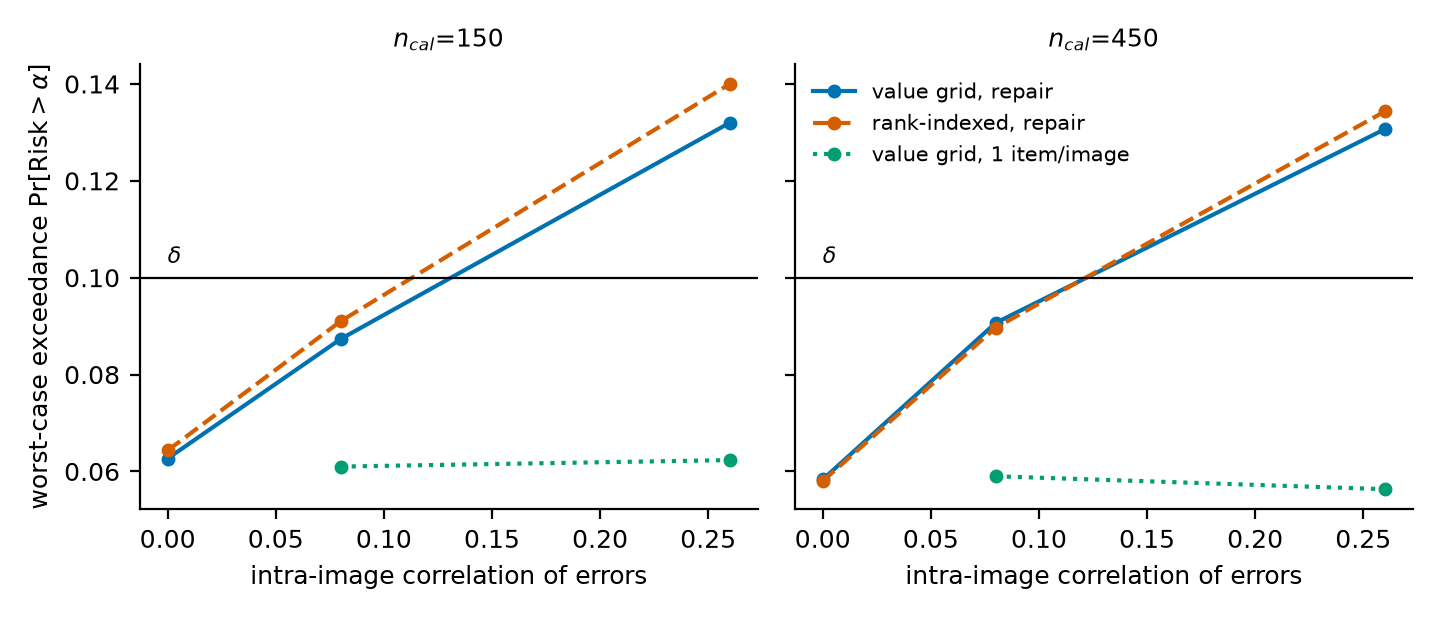
\includegraphics[width=0.95\textwidth]{fig_validity.png}
\caption{Worst-case known-population exceedance over the $\mu$ and $\alpha$ cells, against the intra-image
correlation of errors, with repair. Horizontal line: $\delta=0.10$.}
\label{fig:validity}
\end{figure}

With i.i.d.\ items (ICC $=0$) the exceedance is at most $0.064$ in every cell for both the value-indexed family, which
Theorem~\ref{thm:validity} covers, and the rank-indexed family, which it does not, so the rank-indexed variant is also
conservative here: the missing proof for it is a gap in the argument rather than an observed failure. With positive
within-image correlation the guarantee degrades: at ICC $0.08$ the worst cell is $0.091$, and at ICC $0.26$ the
exceedance of the value-indexed family rises to $0.125$ (filtering) and $0.132$ (repair), above $\delta$, and the rank-indexed
variant to $0.14$. Calibrating on one random item per image restores validity in every cell ($\le0.062$) at the price of a
smaller calibration sample. In the benchmarks used here the measured ICC is slightly negative
(Table~\ref{tab:cohort}), so these data are not in the clustered regime. A benchmark with several correlated questions per image would be, and there the item-level bound
should not be used without the one-item-per-image calibration or a design-effect correction.
